%-----------------------------------
%-----------------------------------
% Beamer template made by Chenxiao
% 2023.11.04 at Qingdao,China
%-----------------------------------
%-----------------------------------

\documentclass[8pt, aspectratio=169]{ctexbeamer}
\setbeameroption{show notes on second screen=bottom}
\mode<presentation> {
	\usetheme{Berlin}
	\usecolortheme{seahorse}
	
	%\setbeamertemplate{footline}
	%若要删除所有幻灯片中的页脚,请取消注释此行
	
	%\setbeamertemplate{footline}[页码]
	%若要用简单的幻灯片计数替换所有幻灯片中的页脚,请取消注释此行
	
	%\setbeamertemplate{导航符号}{}
	%要删除所有幻灯片底部的导航符号,请取消注释此行
}

\usepackage{graphicx} % 允许包含图像
\usepackage{booktabs} % 允许在表中使用\toprule、\ midrule和\ bottomrule
\usepackage[UTF8,noindent]{ctexcap}  % 使用中文输入及显示
\usepackage[bookmarks=true]{hyperref}
\usepackage{mhchem}
\setbeamerfont{footnote}{size=\tiny}
% \usepackage{tikz}
% \usetikzlibrary{shapes,arrows,positioning,calc}
% \usepackage{pgfplots}
% \pgfplotsset{compat=1.18}


\usepackage{siunitx}
\sisetup{
  separate-uncertainty = true,
  inter-unit-product = \ensuremath{{}\cdot{}}
}
% \usepackage{fontspec} % 加载系统字体

% 设置思源宋体
% \setCJKmainfont{Source Han Serif CN} % 简体中文
% %\setCJKmainfont{Source Han Serif TC} % 繁体中文

% % 可选:设置其他字体样式
% \setCJKsansfont{Source Han Sans SC}   % 设置无衬线字体(如标题)
% \setCJKmonofont{Courier New}          % 设置等宽字体


%-----------------------------------
%	以下为正文
%-----------------------------------

\title[光学频谱分析和色彩空间管理初步]{光谱分析和色彩空间管理初步} 
% 简短标题显示在每张幻灯片的底部,完整标题仅在标题页上

\author{Ariel Xiong} % Your name
\institute[浙江工商大学] % 您的机构将出现在每张幻灯片的底部,可能是节省空间的简写
{
	浙江工商大学萨塞克斯人工智能学院 \\ % 你所在的机构
	\medskip
	\textit{ArielHeleneto@outlook.com} % Your email address
}
\date{\today} % 日期,可以更改为自定义日期

\begin{document}

\begin{frame}
	\titlepage % 将标题页打印为第一张幻灯片
\end{frame}

\begin{frame}[allowframebreaks]
	\frametitle{目录} % 目录幻灯片,注释此块以将其删除
	\tableofcontents % 在整个演示过程中,如果您选择使用\ section{}和\ submission{}命令,这些命令将自动打印在此幻灯片上,作为演示的概述
\end{frame}

%-----------------------------------
%	开始创建PPT
%-----------------------------------

\section{光学频谱} % 可以创建章节,以便将您的演讲组织成离散的块,所有章节和小节都会自动打印在目录中,作为演讲的概述
\subsection{光} % 可以在一组具有共同主题的幻灯片之前创建一个小节,以进一步将您的演示分解为块

\begin{frame}
	\frametitle{光的定义}
	\begin{definition}[光]
		光通常指的是人类眼睛可以感受到的电磁波(可见光),视知觉就是对于可见光的知觉。可见光只是电磁波谱上的某一段频谱,一般是定义为波长介于400至700纳米(nm)之间的电磁波,即波长比紫外线长,比红外线短的电磁波。
	\end{definition}
\end{frame}

% \begin{frame}
% 	\frametitle{光的研究史}
% 	TODO)) 光的研究 参考物理教科书
% \end{frame}

\begin{frame}[allowframebreaks]
	\frametitle{光的来源}
	在光的产生过程中,因为跃迁能级的不同,释放出不同频率的光子(爱因斯坦能量方程)。而不同频率的光会有着不同的颜色。
	\begin{table}
		\resizebox{\linewidth}{!}{\begin{tabular}{l l lllllll}
				\toprule
				金属元素 & 锂   & 钠  & 钾\footnote{透过蓝色钴玻璃观察} & 铷  & 钙   & 锶   & 钡   & 铜  \\
				\midrule
				焰色   & 紫红色 & 黄色 & 紫色                    & 紫色 & 砖红色 & 洋红色 & 黄绿色 & 绿色 \\
				\bottomrule
			\end{tabular}}
		\caption{焰色表\footnote{参阅普通高中教科书化学必修第一册第42页表\underline{一些金属元素的焰色}}}
	\end{table}

	\begin{figure}
		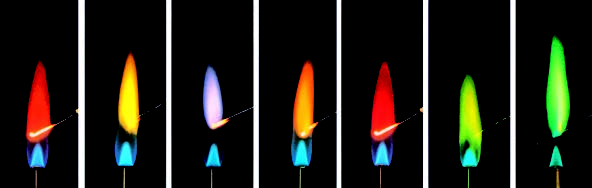
\includegraphics[width=\linewidth]{flametest.png}
		\caption{金属的焰色试验\footnote{参阅普通高中教科书化学必修第一册第42页图2-9}}
	\end{figure}
\end{frame}

\begin{frame}
	\frametitle{激光}
	\begin{definition}[激光]
		激光指透过刺激原子导致电子跃迁释放辐射能量而产生的具有同调性的增强光子束。
	\end{definition}
	处于最低能量状态的原子叫做基态原子。基态原子吸收能量,它的电子会跃迁到较高能级,变为激发态原子。电子从较高能量的激发态跃迁到较低能量的激发态乃至基态时,将释放能量。光(辐射)是电子跃迁释放能量的重要形式。\footnote{普通高中教科书化学选择性必修2物质结构与性质第7页}
\end{frame}

% \begin{frame}
% 	\frametitle{光的物理性质}

% \end{frame}

% 	\begin{frame}
% 		\frametitle{光的化学性质}
% 		TODO)) 参考物理教科书 %https://zh.wikipedia.org/wiki/%E5%85%89#cite_note-Pal2001-2
% 	\end{frame}

% 	\begin{frame}
% 		\frametitle{光的应用}
% 		TODO)) 参考物理教科书 %https://zh.wikipedia.org/wiki/%E5%85%89#cite_note-Pal2001-2
% 	\end{frame}

\subsection{光学频谱}

\begin{frame}[allowframebreaks]
	\frametitle{电磁波谱}
	可见光谱只占有宽广的电磁波谱的一小部分。

	此处定义光包含两侧看不到的部分。
	\begin{figure}
		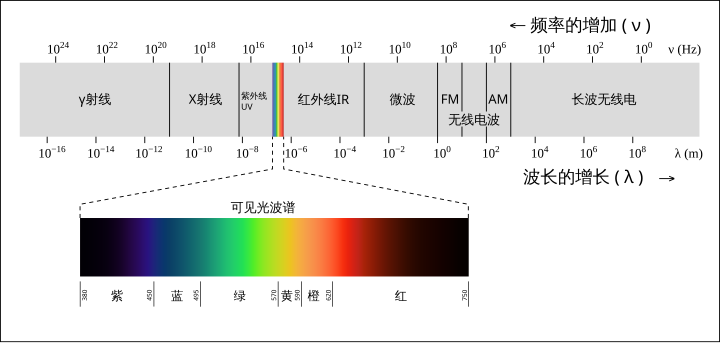
\includegraphics[width=0.7\linewidth]{EM_spectrum_zh-hans.svg.png}
		\caption{可见光谱}
	\end{figure}
\end{frame}

% \begin{frame}
% 	\frametitle{谱}
% 	谱(spectrum)是一种物理情境或现象,其数值不限于一组特定的值,而是可在一段连续区中无间隔地变化。谱的性质又依其是否具连续性或周期性,分为连续谱、离散谱。 
% \end{frame}

\begin{frame}[allowframebreaks]
	\frametitle{光学频谱}
	\begin{definition}[光谱]
		光谱指复色光通过色散系统(如棱镜、光栅)分光后,依光的波长(或频率)的大小顺次排列形成的图案。
	\end{definition}
	% \begin{figure}
	% 	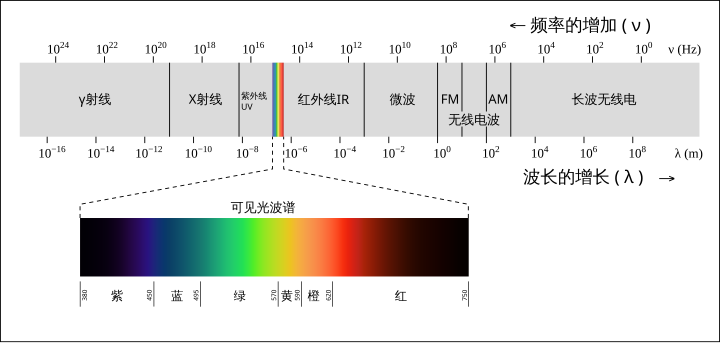
\includegraphics[width=\linewidth]{EM_spectrum_zh-hans.svg.png}
	% 	\caption{可见光谱}
	% \end{figure}
	\begin{figure}
		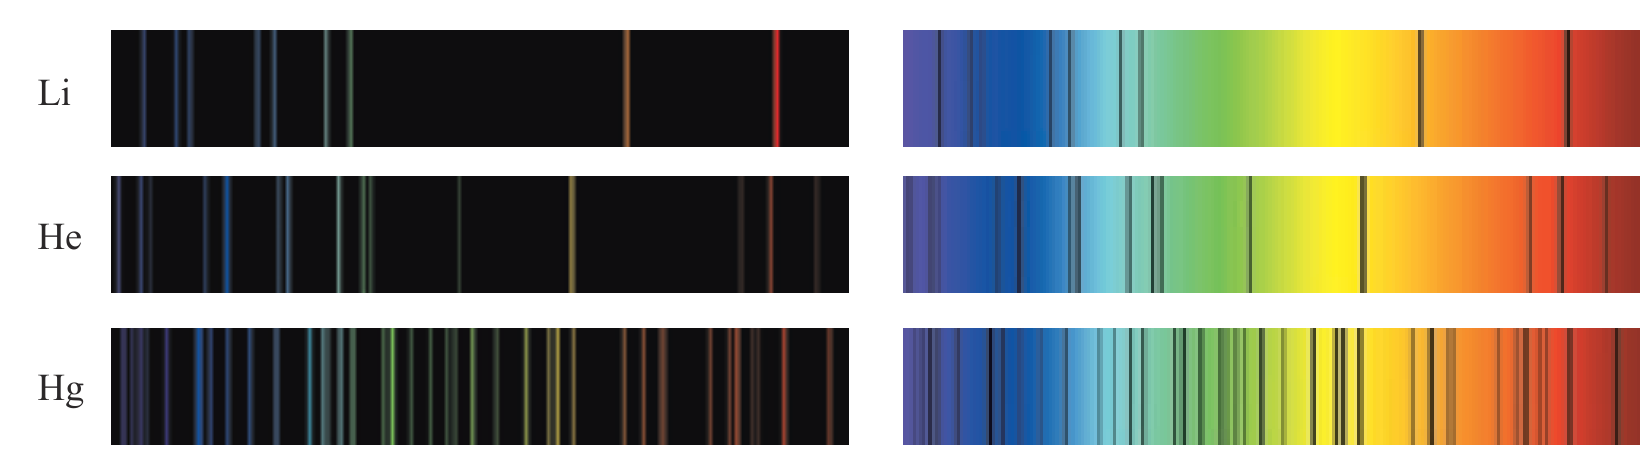
\includegraphics[width=\linewidth]{guangpu.png}
		\caption{$\ce{Li}$、$\ce{He}$、$\ce{Hg}$的发射光谱(左)和吸收光谱(右)}
	\end{figure}
	\note{发射光谱有的物体能自行发光,由它直接产生的光形成的光谱叫做发射光谱。发射光谱可分为三种不同类别的光谱:线状光谱、带状光谱和连续光谱。

		吸收光谱在连续光谱中某些波长的光被物质吸收后产生的光谱被称作吸收光谱。

		散射光谱当光照射到物质上时,会发生非弹性散射,在散射光中除有与激发光波长相同的弹性成分(瑞利散射)外,还有比激发光波长长的和短的成分,后一现象统称为拉曼效应。这种产生新波长的光的散射被称为拉曼散射,所产生的光谱被称为拉曼光谱或拉曼散射光谱。}
	%https://zh.wikipedia.org/wiki/%E5%85%89%E8%B0%B1
\end{frame}

% 	\begin{frame}
% 		\frametitle{光学定义}


% 	%https://zh.wikipedia.org/wiki/%E5%85%89%E8%B0%B1
% 	\end{frame}

% 	\begin{frame}
% 		\frametitle{光的折射和光谱}
% 		复色光中有着各种波长(或频率)的光,这些光在介质中有着不同的折射率。因此,当复色光通过具有一定几何外形的介质(如三棱镜)之后,波长不同的光线会因出射角的不同而发生色散现象,投映出连续的或不连续的彩色光带。

% 这个原理亦被应用于著名的太阳光的色散实验。太阳光呈现白色,当它通过三棱镜折射后,将形成由红、橙、黄、绿、蓝、靛、紫(或红、橙、黄、绿、青、蓝、紫)顺次连续分布的彩色光谱,覆盖了大约在390到770纳米的可见光区。历史上,这一实验由英国科学家艾萨克·牛顿爵士于1666年完成,使得人们第一次接触到了光的客观的和定量的特征。 

% 	%https://zh.wikipedia.org/wiki/%E5%85%89%E8%B0%B1
% 	\end{frame}

% 	\begin{frame}
% 		\frametitle{按产生方式分类光谱}

% 		    发射光谱Emission:有的物体能自行发光,由它直接产生的光形成的光谱叫做发射光谱。发射光谱可分为三种不同类别的光谱:线状光谱、带状光谱和连续光谱。
%     吸收光谱Absorption:在连续光谱中某些波长的光被物质吸收后产生的光谱被称作吸收光谱。
%     散射光谱Scattering:当光照射到物质上时,会发生非弹性散射,在散射光中除有与激发光波长相同的弹性成分(瑞利散射)外,还有比激发光波长长的和短的成分,后一现象统称为拉曼效应。这种产生新波长的光的散射被称为拉曼散射,所产生的光谱被称为拉曼光谱或拉曼散射光谱。
% 		按产生方式,光谱可分为发射光谱、吸收光谱和散射光谱。

% 有的物体能自行发光,由它直接产生的光形成的光谱叫做发射光谱。

% 发射光谱可分为三种不同类别的光谱:线状光谱、带状光谱和连续光谱。线状光谱主要产生于原子,由一些不连续的亮线组成;带状光谱主要产生于分子,由一些密集的某个波长范围内的光组成;连续光谱则主要产生于白炽的固体、液体或高压气体受激发发射电磁辐射,由连续分布的一切波长的光组成。


% 在白光通过气体时,气体将从通过它的白光中吸收与其特征谱线波长相同的光,使白光形成的连续谱中出现暗线。此时,这种在连续光谱中某些波长的光被物质吸收后产生的光谱被称作吸收光谱。通常情况下,在吸收光谱中看到的特征谱线会少于线状光谱。

% 当光照射到物质上时,会发生非弹性散射,在散射光中除有与激发光波长相同的弹性成分(瑞利散射)外,还有比激发光波长长的和短的成分,后一现象统称为拉曼效应。这种现象于1928年由印度科学家拉曼所发现,因此这种产生新波长的光的散射被称为拉曼散射,所产生的光谱被称为拉曼光谱或拉曼散射光谱。
% 	%https://zh.wikipedia.org/wiki/%E5%85%89%E8%B0%B1
% 	\end{frame}

\section{色彩空间}

\subsection{颜色}

\begin{frame}
	\frametitle{颜色}

	颜色又称色彩、色泽,是眼、脑和我们的生活经验对光的颜色类别描述的视觉感知特征。这种对颜色的感知来自可见光谱中的电磁辐射对人眼视锥细胞的刺激。颜色是由光反射所产生的,这种反射是由物体的物理性质决定的,如光的吸收、发射光谱等。
\end{frame}

\begin{frame}
	\frametitle{单色和混合色}

	\note{大多数光源的光谱不是单色的,它们的光是由不同强度和波长的光混合组成的。人眼将许多这样的混合光的颜色与单色光源的光的颜色看成是同样。比如上面表格中的橙色,实际上就不是单色的600奈米的光,实际上它是由红色和绿色的光混合组成的(显示器无法产生单色的橙色)。出于眼睛的生理原理,我们无法区分这两种光的颜色。

		也有许多颜色是不可能是单色的,因为没有这样的单色的颜色。比如说黑色、灰色和白色就是这样的颜色,粉红色或淡紫色也是这样的颜色。 }

\end{frame}

\subsection{理想色彩空间}

\begin{frame}
	\frametitle{光学频谱密度}
	令 $dI_\lambda$ 为一束光波长在 $[ \lambda , \lambda+d\lambda ]$区间的光强,则单位波长区间的光强是$i(\lambda) =\frac{dI_\lambda}{d\lambda}$ 称作谱密度。在现代化学中,常利用原子光谱上的特征谱线来鉴定元素,称为光谱分析。

	%https://zh.wikipedia.org/wiki/%E5%85%89%E8%B0%B1
\end{frame}

\subsection{色彩空间设计}

\begin{frame}[allowframebreaks]
	\frametitle{色彩匹配实验}

	\begin{columns}
		\column{0.5\textwidth}
		我们知道不同的色光混合起来会产生其他的颜色,这其实是人眼的一种生理反应。为了了解到底人眼是怎么融合不同颜色色光的,有人设计了一个实验来定量测量到底参入多少红、绿、蓝三原色会让人眼觉得待测色光和三色光混合色感觉完全一样。实验原理如 \autoref{fig:exp} 所示。


		\column{0.5\textwidth}
		\begin{figure}
			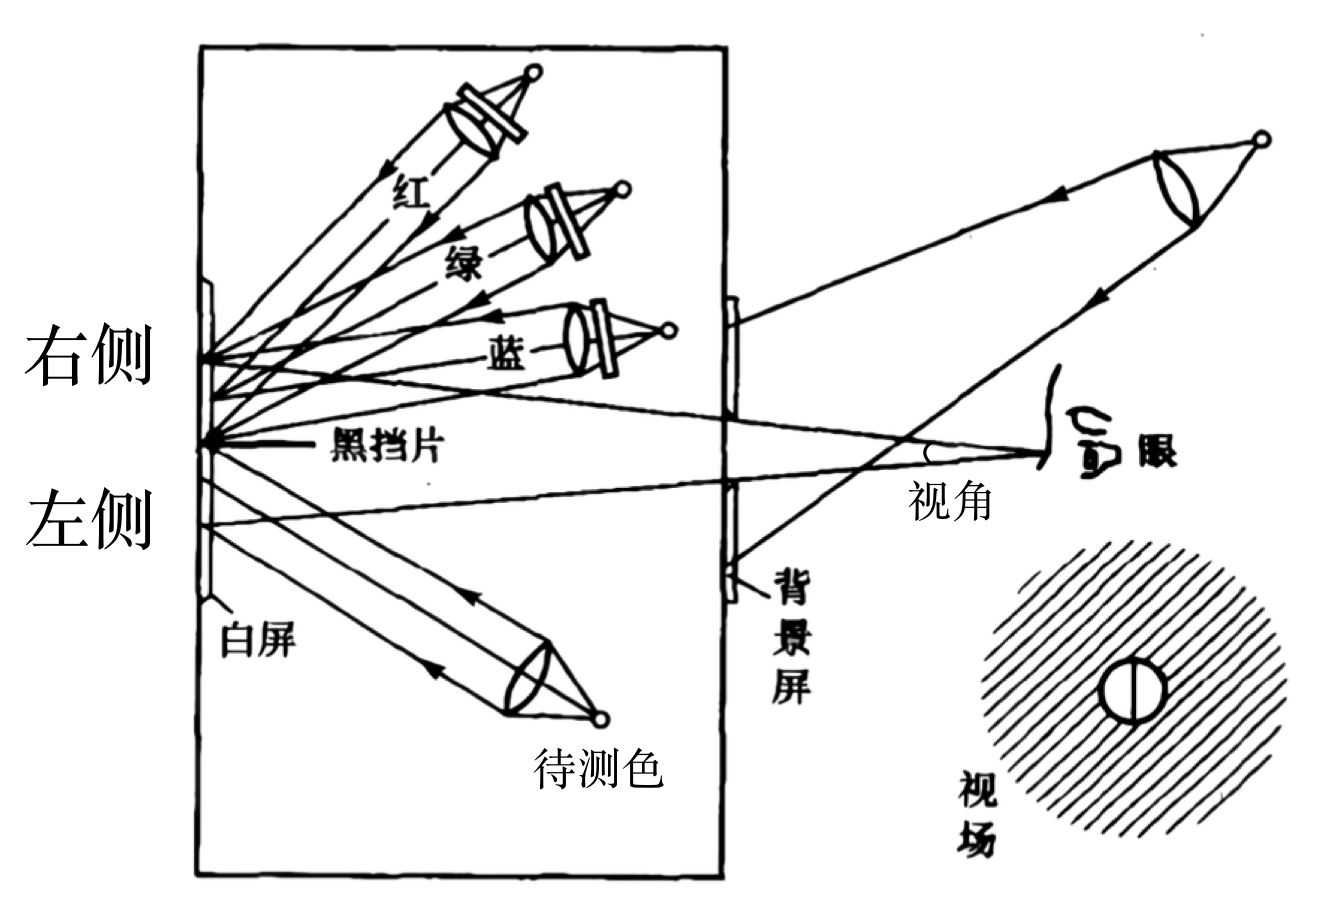
\includegraphics[width=\linewidth]{exp.png}
			\caption{实验原理}
			\label{fig:exp}
		\end{figure}
	\end{columns}

	\newpage

	\begin{columns}
		\column{0.5\textwidth}
		其中 R 为 $\SI{700}{nm}$,G 为 $\SI{546.1}{nm}$, B 为 $\SI{435.8}{nm}$。

		实验结果如 \autoref{fig:expres} 所示。


		\column{0.5\textwidth}
		\begin{figure}
			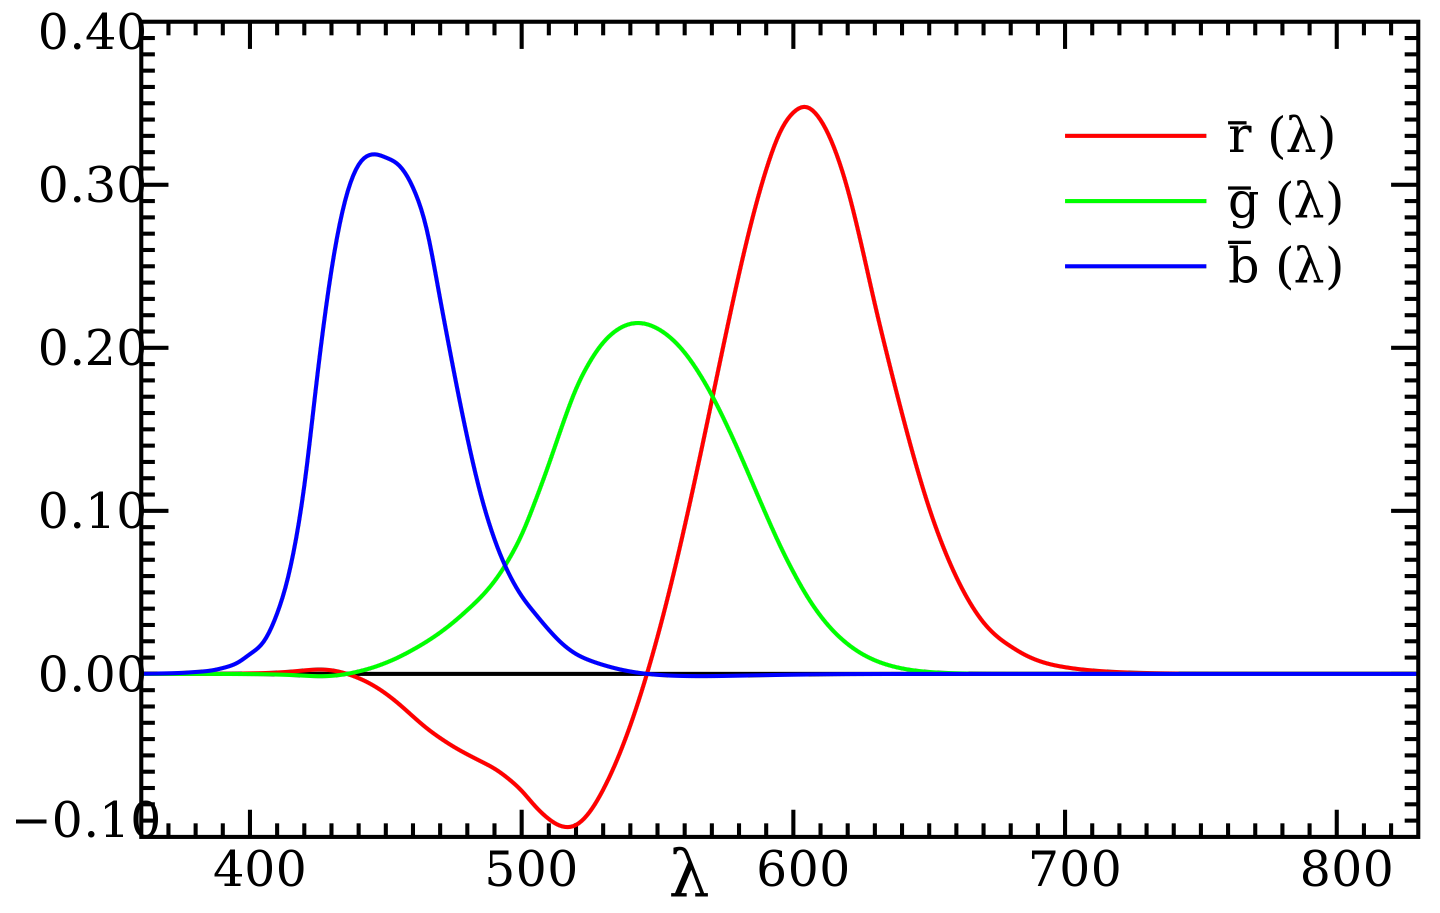
\includegraphics[width=\linewidth]{ciji.png}
			\caption{光谱三刺激值曲线图}
			\label{fig:expres}
		\end{figure}
	\end{columns}


\end{frame}

\begin{frame}
	\frametitle{CIE 1931-RGB 色度系统}

	\begin{columns}
		\column{0.5\textwidth}
		根据 \autoref{fig:expres} 的结果,使用 $r=\frac{\overline{r}}{\overline{r}+\overline{g}+\overline{b}}$, $g=\frac{\overline{g}}{\overline{r}+\overline{g}+\overline{b}}$ 作图如 \autoref{fig:cie1931rgb} 所示。

		$rg=(0,0)$ 于 $\SI{435.8}{nm}$,通过 $rg=(0,1)$ 于$\SI{546.1}{nm}$,通过 $rg=(1,0)$ 于 $\SI{700}{nm}$。

		\column{0.5\textwidth}
		\begin{figure}
			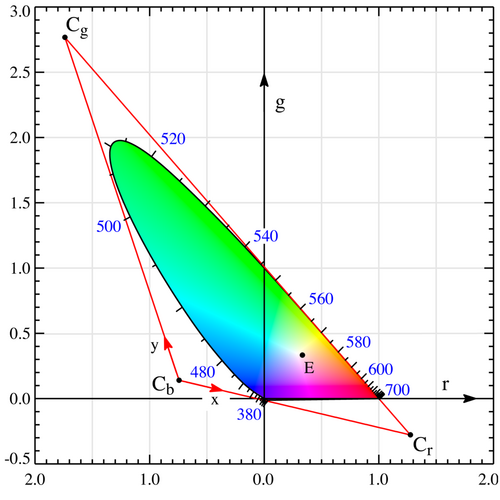
\includegraphics[width=0.6\linewidth]{cie1931.png}
			\caption{CIE rg色度图}
			\label{fig:cie1931rgb}
		\end{figure}
	\end{columns}

\end{frame}

\begin{frame}
	\frametitle{CIE 1931 XYX 色度系统}
	\begin{columns}
		\column{0.5\textwidth}
		对 \autoref{fig:cie1931rgb} 作几何变换,得到 \autoref{fig:cie1931xy}。
		\column{0.5\textwidth}
		\begin{figure}
			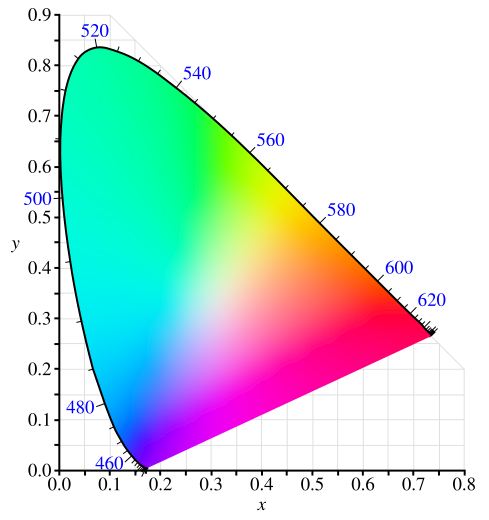
\includegraphics[width=0.6\linewidth]{cie1931xy.png}
			\caption{CIE xy色度图}
			\label{fig:cie1931xy}
		\end{figure}
	\end{columns}


\end{frame}
\begin{frame}

\end{frame}


\begin{frame}
	\frametitle{色彩空间}
	色彩空间,是对色彩的组织方式。借助色彩空间和针对物理设备的测试,可以得到色彩的固定模拟和数字表示。色彩空间可以只通过任意挑选一些颜色来定义,比如像彩通系统就只是把一组特定的颜色作为样本,然后给每个颜色定义名字和代码;也可以是基于严谨的数学定义,比如 Adobe RGB、sRGB。

	样本法:$\ce{MnO4^-}$ 紫色、$\ce{Cu^2+}$ 浅蓝色、$\ce{Fe^2+}$ 浅绿色、$\ce{Fe^3+}$ 黄色、$\ce{Cr^2+}$ 黄色、$\ce{Cr^3+}$ 绿色、$\ce{Cr2O7^2+}$ 橙色、$\ce{CrO4^2-}$ 黄色、$\ce{[Fe(SCN)x]^{3-x}}$ 血红色。

	%https://zh.wikipedia.org/wiki/%E5%85%89%E8%B0%B1 三色刺激值 https://zh.wikipedia.org/wiki/CIE_1931%E8%89%B2%E5%BD%A9%E7%A9%BA%E9%97%B4
\end{frame}
\begin{frame}
	\frametitle{色彩模型}

	色彩模型(英语:Color model)是一种抽象数学模型,通过一组数字来描述颜色(例如RGB使用三元组、CMYK使用四元组)。如果一个色彩模型与绝对色彩空间没有映射关系,那么它多少都是与特定应用要求几乎没有关系的任意色彩系统。

	%https://zh.wikipedia.org/wiki/%E5%85%89%E8%B0%B1 三色刺激值 https://zh.wikipedia.org/wiki/CIE_1931%E8%89%B2%E5%BD%A9%E7%A9%BA%E9%97%B4
\end{frame}

\begin{frame}
	\frametitle{RGB}

	\begin{columns}
		\column{0.5\textwidth}
		RGB采用加法混色法,因为它是描述各种“光”通过何种比例来产生颜色。光线从暗黑开始不断叠加 产生颜色。RGB描述的是红绿蓝三色光的数值。RGBA是在RGB上增加阿尔法通道实现透明效果。

		\column{0.5\textwidth}
		\begin{figure}
			\includegraphics[width=0.6\linewidth]{srgb.png}
			\caption{sRGB 色度图}
		\end{figure}
	\end{columns}



	%https://zh.wikipedia.org/wiki/%E5%85%89%E8%B0%B1 三色刺激值 https://zh.wikipedia.org/wiki/CIE_1931%E8%89%B2%E5%BD%A9%E7%A9%BA%E9%97%B4
\end{frame}

\begin{frame}
	\frametitle{印刷四分色模式}
	印刷四分色模式(CMYK color model)是彩色印刷时采用的一种套色模式,利用色料的三原色混色原理,加上黑色油墨,共计四种颜色混合叠加,形成所谓“全彩印刷”。四种标准颜色是:

	C:Cyan  青色或“水蓝”

	M:Magenta  洋红色或“紫色”

	Y:Yellow 黄色

	K:Key plate 黑色。

	%https://zh.wikipedia.org/wiki/%E5%85%89%E8%B0%B1 三色刺激值 https://zh.wikipedia.org/wiki/CIE_1931%E8%89%B2%E5%BD%A9%E7%A9%BA%E9%97%B4
\end{frame}

\begin{frame}
	\frametitle{HSL}
	\begin{columns}
		\column{0.5\textwidth}
		HSV(色相、饱和度、明度),是艺术家们常用的,因为与加法减法混色的术语相比,使用色相、饱和度等概念描述色彩更自然直观。

		HSL(色相、饱和度、亮度),与HSV非常相似,仅用亮度(Lightness)替代了明度(Brightness)。二者区别在于,一种纯色的明度等于白色的明度,而纯色的亮度等于中度灰的亮度。

		\column{0.5\textwidth}
		\begin{figure}
			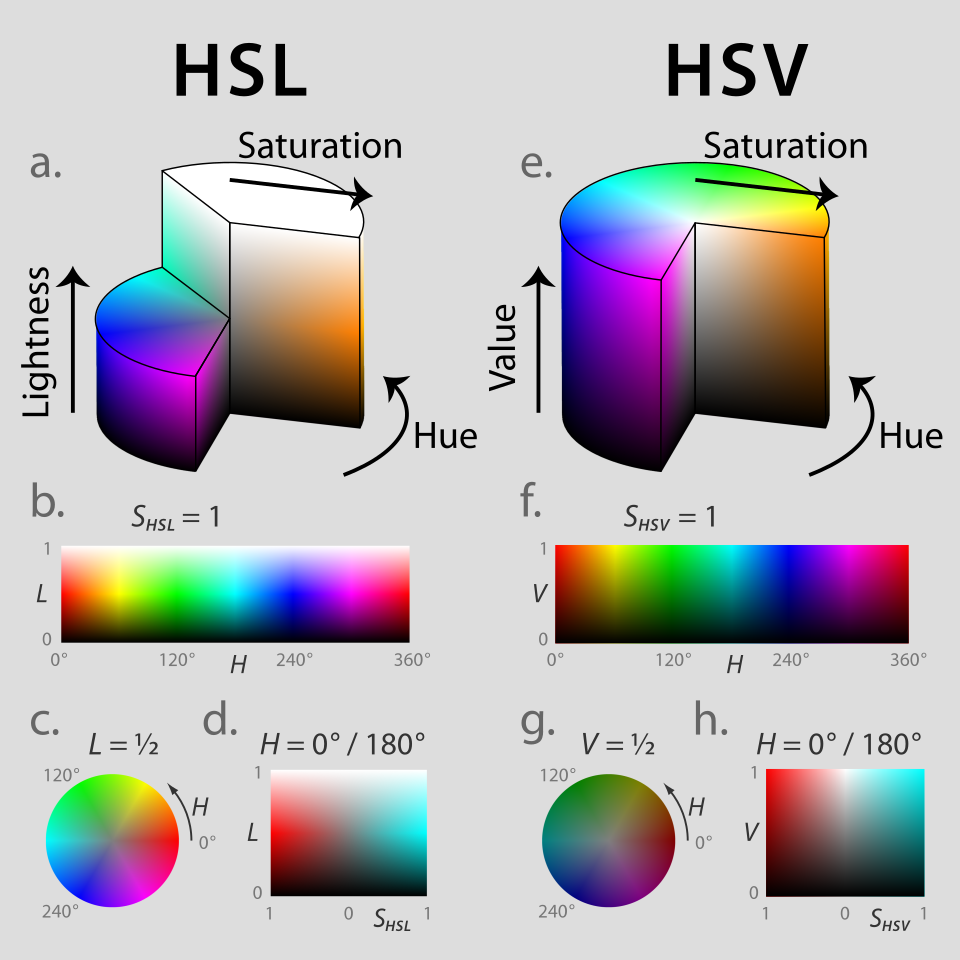
\includegraphics[width=0.7\linewidth]{hsl.png}
			\caption{HSL 色度图}
		\end{figure}
	\end{columns}
\end{frame}
% 	\begin{frame}
% 		\frametitle{PID 系统}
% 		\begin{figure}
% 			\resizebox{\linewidth}{!}{
% 				\begin{tikzpicture}[
%     block/.style={draw, rectangle, minimum height=1cm, minimum width=2cm, align=center},
%     sum/.style={draw, circle, minimum size=6mm},
%     input/.style={coordinate},
%     output/.style={coordinate},
%     arrow/.style={->, >=stealth', thick},
%     node distance=1cm
% ]

% % 输入节点
% \node[input] (setpoint) {};
% \node[left=0.1cm of setpoint] {$r(t)$};

% % 第一个求和点 (误差计算)
% \node[sum, right=of setpoint] (sum1) {$\Sigma$};
% % \node[above left=0.1cm and 0.1cm of sum1] {$+$};
% % \node[below left=0.1cm and 0.1cm of sum1] {$-$};

% % 分支点 (误差信号)
% \node[circle, inner sep=0pt, minimum size=2pt, fill=black, right=1cm of sum1] (branch) {};

% % PID 控制器内部结构
% % 比例支路
% \node[block, above right=1cm and 2cm of branch] (p) {$K_p$};
% % \node[above=0.1cm of p] {比例支路};

% % 积分支路
% \node[block, right=2cm of branch] (i) {$\displaystyle\frac{K_i}{s}$};
% % \node[above=0.1cm of i] {积分支路};

% % 微分支路
% \node[block, below right=1cm and 2cm of branch] (d) {$K_d s$};
% % \node[below=0.1cm of d] {微分支路};

% % PID 求和点
% \node[sum, right=7cm of branch] (sum2) {$\Sigma$};

% % 被控对象
% \node[block, right=of sum2] (plant) {$G(s)$};

% % 输出节点
% \node[output, right=of plant] (output) {};
% \node[right=0.1cm of output] {$y(t)$};

% % 反馈回路
% \node[block, below= 2.5cm of plant] (feedback) {$H(s)$};

% % 第二个求和点 (反馈信号)
% \node[sum, left= 2cm of feedback] (sum3) {$\Sigma$};

% % 连接线
% % 前向通道
% \draw[arrow] (setpoint) -- node[above, pos=0.8] {$+$} (sum1);
% \draw[arrow] (sum1) -- node[above] {$e(t)$} (branch);
% \draw[arrow] (branch) |- (p);
% \draw[arrow] (branch) -- (i);
% \draw[arrow] (branch) |- (d);
% \draw[arrow] (p) -| node[above,pos=0.25] {$K_p e(t)$} (sum2);
% \draw[arrow] (i) -- node[above] {$\displaystyle K_i \int e(t) dt$} (sum2);
% \draw[arrow] (d) -| node[above,pos=0.25] {$K_d \frac{de(t)}{dt}$} (sum2);
% \draw[arrow] (sum2) -- node[above] {$u(t)$} (plant);
% \draw[arrow] (plant) -- (output);

% % 反馈通道
% \draw[arrow] (output) |- (feedback);
% \draw[arrow] (feedback) -- node[above] {$y_m(t)$} (sum3);
% \draw[arrow] (sum3) -| node[pos=0.99, left] {$-$} (sum1);

% % 连接反馈求和点
% % \draw[arrow] (branch) |- (sum3) node[pos=0.25, right] {$e(t)$};

% % 标注
% \draw[dashed] ($(branch)+(-0.5,-2.5)$) rectangle ($(sum2)+(0.5,2.5)$);
% % \node[above] at ($(branch)!0.5!(sum2)+(0,1.8)$) {PID控制器};

% % 系统标签
% % \node[above=0.5cm of plant] {PID控制系统框图};
% % \node[below=1cm of feedback] {负反馈回路};

% \end{tikzpicture}
% 			}
% 			\caption{PID 控制器}
% 		\end{figure}
% 	\end{frame}

% 	\subsection{拉普拉斯变换和傅里叶变换}

% 	\begin{frame}
% 		\frametitle{拉普拉斯变换}
% 		\begin{definition}[拉普拉斯变换]
% 			信号或函数 $f$ 的拉普拉斯变换(定义于 $t \geq 0$)是函数 $$F(s) = \mathcal{L}\{f(t)\} = \int_0^{\infty} f(t)e^{-st} dt$$
% 		\end{definition}
% 		\begin{figure}[width=\linewidth]

% 		\end{figure}
% 	\end{frame}

% 	\begin{frame}
% 		\frametitle{傅里叶变换}
% 		\begin{definition}[傅里叶变换]
% 			信号或函数 $f$ 的傅里叶变换是函数 $$F(\omega) = \mathcal{F}\{f(t)\} = \int_{-\infty}^{\infty} f(t)e^{-j\omega t} dt$$
% 		\end{definition}
% 		\begin{figure}[width=\linewidth]

% 		\end{figure}
% 	\end{frame}

% 	\section{数字信号处理初步}
% 	\subsection{定义}
% 	\begin{frame}
% 		\frametitle{信号的性质}
% 		\begin{definition}[信号]
% 			携带信息的量。
% 		\end{definition}
% 		\begin{definition}[模拟信号]
% 			用连续变量物理量表示的信号。
% 		\end{definition}
% 		\begin{definition}[数字信号]
% 			用物理量的离散值表示的信号。
% 		\end{definition}
% 		\note{模拟信号:电压

% 		常见的数字信号:数字式电压表量出来的值

% 		需要注意的是,这里的数字信号不一定只能是0和1		
% 	}
% 	\end{frame}

% 	\begin{frame}[allowframebreaks]
% 		\frametitle{常见的数字信号}
% 		\begin{definition}[冲激信号]
% 			\begin{equation}
% 				\delta [n]=\begin{cases}
% 					1 (n=0)\\0 (n\neq 0)
% 				\end{cases}
% 			\end{equation}
% 		\end{definition}

% 		\begin{definition}[阶跃信号]
% 			\begin{equation}
% 				u[n]=\begin{cases}
% 					1 (n\geq0)\\0 (n< 0)
% 				\end{cases}
% 			\end{equation}
% 		\end{definition}
% 		\begin{definition}[斜坡信号]
% 			\begin{equation}
% 				r[n]=\begin{cases}
% 					n (n\geq0)\\0 (n< 0)
% 				\end{cases}
% 			\end{equation}
% 		\end{definition}

% 	\end{frame}

% 	\begin{frame}[allowframebreaks]
% 		\frametitle{冲击响应}
% 		\begin{definition}[冲激响应]
% 			当系统的输入为冲击信号时,输出为该系统的冲激响应,用 $h[n]$ 表示。
% 		\end{definition}
% 	\end{frame}

% 	\subsection{采样}

% 	\begin{frame}
% 		\frametitle{模数转换}

% 		将模拟信号转换为数字信号通常需要 ADC 组件。该组件一般公式如下。

% 		$$\mathbf{output}=\frac{\mathbf{input}}{\mathbf{range}}\times{2^\mathbf{bit}}$$
% 	\end{frame}

% \begin{frame}
% 	\frametitle{模数转换}
% 	将模拟信号转换为数字信号通常需要 ADC 组件。该组件一般公式如下。
% 	\begin{definition}[香农采样定理]
% 		包含最高频率 $f_c$ 成分的模拟信号可以完全用样本表示,前提是采样率 $f_s\geq2f_c$。
% 	\end{definition}
% \end{frame}

% 	\begin{frame}
% 		\frametitle{香农采样定理}
% 		\begin{definition}[香农采样定理]
% 			包含最高频率 $f_c$ 成分的模拟信号可以完全用样本表示,前提是采样率 $f_s\geq2f_c$。
% 		\end{definition}
% 	\end{frame}

% 	\begin{frame}
% 		\frametitle{混叠}
% 		\begin{figure}
% 			\resizebox{0.9\linewidth}{!}{
% 				\begin{tikzpicture}[scale=0.03]
% \begin{axis}[
%     axis lines = middle,
%     xmin = 0, xmax = 2,
%     ymin = -1.25, ymax = 1.25,
%     xlabel = $t$,
%     ylabel = {$f(t)$},
% ]
% \addplot [
%     domain=0:2,
%     samples=10000,
%     color=blue,
% ]
% {sin(deg(x*4*pi))};
% \addplot [
%     domain=0:2,
%     samples=7,
%     color=red,
% ]
% {sin(deg(x*4*pi))};
% \end{axis}
% \end{tikzpicture}
% 			}
% 			\caption{采样率影响}
% 		\end{figure}
% 	\end{frame}

% 	\subsection{傅里叶变换}

% 	\begin{frame}
% 		\frametitle{傅里叶变换}
% 		\begin{definition}[傅里叶变换]
% 			对于数字信号 $x[n]$,其傅里叶变换为 $$X(\omega)=\sum_{-\infty}^{\infty}x[n]e^{-j\omega n}$$。其中,$\omega\in [0,2\pi]$。
% 		\end{definition}
% 	\end{frame}

% 	\begin{frame}
% 		\frametitle{傅里叶变换的性质}
% 		\begin{itemize}
% 			\item 线性
% 			\item 时移:$x[n-n_0]\rightarrow X(\omega)e^{-j\omega n_0}$
% 			\item 卷积:$x_1[n]*x_2[n]\rightarrow X_1(\omega)\times X_2(\omega)$
% 		\end{itemize}
% 	\end{frame}

% 	\begin{frame}
% 		\frametitle{离散傅里叶变换}
% 		\begin{definition}[离散傅里叶变换]
% 			对于长度为 $N$ 的序列,其离散傅里叶变换为 $$X[k]=\sum_0^{N-1}x[n]e^{-j\frac{2\pi k n}{N}}$$
% 		\end{definition}
% 	\end{frame}

% 	\subsection{数字系统}

% 	\begin{frame}
% 		\frametitle{线性时不变系统}
% 		\begin{definition}[线性系统]
% 			如果一个系统满足线性性质,那么对于任意输入信号 $x_{1}(t)$ 和 $x_{2}(t)$,以及任意常数 $a$ 和 $b$,如果输入为 $ax_{1}(t)+bx_{2}(t)$,则输出为 $ay_{1}(t)+by_{2}(t)$,其中 $y_{1}(t)$ 和 $y_{2}(t)$ 分别是输入 $x_{1}(t)$ 和 $x_{2}(t)$ 的响应。
% 		\end{definition}
% 		\begin{definition}[时不变系统]
% 			如果一个系统满足时不变性质,那么对于任意输入信号 $x(t)$ 和任意时间延迟 $\tau$,如果输入为 $x(t-\tau)$,则输出为 $y(t-\tau )$,其中 $y(t)$ 是输入 $x(t)$ 的响应。
% 		\end{definition}
% 	\end{frame}

% 	\begin{frame}
% 		\frametitle{线性时不变系统的描述}
% 		\begin{definition}[线性时不变系统]
% 			$$y[n]=\sum_{k=1}^{N}a_k y[n-k]+\sum_{k=1}^{N}b_k x[n-k]$$
% 		\end{definition}
% 	\end{frame}

% 	\begin{frame}
% 		\frametitle{因果系统}
% 		% 因果系统是指
% 		\begin{definition}[因果]
% 			因果系统,称一个系统是“因果”的,是指此系统满足因果性。即对输入的响应不可能在此输入到达的时刻之前出现;也就是说系统的输出仅与当前与过去的输入有关,而与将来的输入无关。
% 		\end{definition}
% 	\end{frame}

% 	\begin{frame}
% 		\frametitle{转换模拟信号到数字信号}
% 		\begin{itemize}
% 			\item $y(t)$ 转换为 $y[n]$。
% 			\item $x(t)$ 转换为 $x[n]$。
% 			\item $\frac{dy(t)}{dt}$ 转换为 $\frac{y[n]-y[n-1]}{T}$。
% 			\item $\frac{dy^2(t)}{dt^2}$ 转换为 $\frac{\frac{y[n]-y[n-1]}{T}-\frac{y[n-1]-y[n-2]}{T}}{T}$。
% 		\end{itemize}
% 	\end{frame}

% 	\subsection{门限法}

% 	\begin{frame}
% 		\frametitle{门限法滤噪音}
% 		将傅里叶变换后幅度低于一定值的噪声幅度调整为$0$,然后还原原始信号。
% 	\end{frame}

% 	\begin{frame}
% 		\frametitle{短时距傅里叶变换}
% 		计算短时距傅里叶变换的过程是将长时间信号分成数个较短的等长信号,然后再分别计算每个较短段的傅里叶变换。通常拿来描绘频域与时域上的变化,为时频分析中其中一个重要的工具。 
% 		\begin{definition}[短时距傅里叶变换]
% 			对于数字信号 $x[n]$,其短时距傅里叶变换为 $$\mathbf{STFT}\{x[n]\}(m,\omega)\equiv X(m,\omega) = \sum_{n=-\infty}^{\infty} x[n]w[n-m]e^{-j \omega n} $$。其中,$\omega\in [0,2\pi]$。
% 		\end{definition}
% 	\end{frame}

% 	\section{滤波器设计}

% 	\subsection{Z 变换}

% 	\begin{frame}
% 		\frametitle{Z 变换}
% 		\begin{definition}[Z 变换]
% 			对于数字信号 $x[n]$,其 Z 变换为 $$X(\mathcal{Z})=\sum_0^{\infty}x[n]\mathcal{Z}^{-n}$$。其中,$\mathcal{Z}$ 为一复数。
% 		\end{definition}

% 		注意到,当 $\mathcal{Z}=e^{j\omega}$ 时,该变换退化为傅里叶变换。
% 		% \note{练习:将$x[n]=\{1,0.8,0.8^2,\cdots,0.8^n$转化为}
% 	\end{frame}
% 	\begin{frame}[allowframebreaks]
% 		\frametitle{Z 变换练习}
% 		\begin{problem}
% 			求数字信号 $x[n]=\left\{1,0.8,0.8^2,\cdots,0.8^n\right\}$ 的 Z 变换。
% 		\end{problem}
% 		\begin{solution}
% 			\begin{equation*}\begin{aligned}
% X(\mathcal{Z}) =& \sum_0^{\infty}x[n]\mathcal{Z}^{-n} & \\
% = & \left(0.8\mathcal{Z}^-1\right)^0+\left(0.8\mathcal{Z}^-1\right)^1+\left(0.8\mathcal{Z}^-1\right)^2+\cdots\left(0.8\mathcal{Z}^-1\right)^n \\
% =& \lim_{n\rightarrow\infty}\frac{1-\cdots\left(0.8\mathcal{Z}^-1\right)^n}{1-0.8\mathcal{Z}^-1} \\
% =& \frac{z}{z-0.8}
% \end{aligned}\end{equation*}
% 		\end{solution}

% 	\end{frame}
% 	\begin{frame}
% 			\frametitle{时移信号的 Z 变换}
% 			\begin{equation*}
% 				\begin{aligned}
% {} & \sum_{n=0}^{\infty}x[n-1]u[n-1]\mathcal{Z}^{-n}  \\
% =& x[-1]u[-1]\mathcal{Z}^0+x[0]\mathcal{Z}^{-1}+x[1]\mathcal{Z}^{-2}+x[2]\mathcal{Z}^{-3}+\cdots \\
% =& \mathcal{Z}^{-1}(x[0]\mathcal{Z}^0+x[1]\mathcal{Z}^{-1}+x[2]\mathcal{Z}^{-2}+\cdots) \\
% =& \mathcal{Z}^{-1}X(\mathcal{Z})
% \end{aligned}
% 			\end{equation*}

% \begin{definition}[Z 变换]
% 	对于数字信号 $x[n]$,其 Z 变换为 $$X(\mathcal{Z})=\sum_0^{\infty}x[n]z^{-n}$$。其中,$z$ 为一复数。
% \end{definition}

% 注意到,当 $z=e^{j\omega}$ 时,该变换退化为傅里叶变换。
% 	\end{frame}
% 	\subsection{传递函数和系统稳定性}
% 	\begin{frame}
% 			\frametitle{传递函数}
% 			\begin{definition}[传递函数]
% 			对于一个输出为$y[n]$,输入为$x[n]$的系统,其传递函数为$H(\mathcal{Z})=\frac{Y(\mathcal{Z})}{X(\mathcal{Z})}$。
% 		\end{definition}
% 	\end{frame}
% 	\begin{frame}
% 			\frametitle{系统稳定性}
% 			\begin{definition}[系统稳定性]
% 			$\lim_{n\rightarrow\infty}h[n]=0$ 的系统为稳定系统。$\lim_{n\rightarrow\infty}h[n]=a\neq0$ 的系统为临界稳定系统。 
% 			\end{definition}
% 	\end{frame}
% 	\begin{frame}
% 			\frametitle{零点和极点}
% 			\begin{definition}[零点]
% 			使传递函数分子取得 $0$ 的 $\mathcal{Z}$ 的取值称为零点。
% 			\end{definition}
% 			\begin{definition}[极点]
% 			使传递函数分母取得 $0$ 的 $\mathcal{Z}$ 的取值称为零点。
% 			\end{definition}
% 	\end{frame}
% 	\begin{frame}
% 			\frametitle{零点和极点的性质}
% 			在零点上增益总是 $0$,在极点上增益取得最大值。
% 	\end{frame}
% 	\begin{frame}
% 			\frametitle{判断系统稳定性}
% 			极点的模小于  $1$。
% 	\end{frame}
% 	\subsection{滤波器设计}
% 	\begin{frame}[allowframebreaks]
% 			\frametitle{练习设计一个滤波器}
% 			\begin{problem}
% 				一个电子设备需要配备一个数字滤波器,用于阻止 $\SI{250}{Hz}$ 的频率并允许 $\SI{500}{Hz}$ 的频率通过。采样率为 $\SI{2000}{Hz}$。
% 在 $\mathcal{Z}$ 平面中,选择并显示一对零点和一对极点的位置,
% 增益为 $25$,位于通过频率处。绘制从 0 到采样频率一半范围内的频率响应图,并标记任何具有特殊意义的值。
% 			\end{problem}
% 			\begin{solution}
% 				\begin{itemize}
% 					\item 确定传递函数:$H(\mathcal{Z})=\frac{\left(\mathcal{Z}-1\angle \frac{\pi}{4}\right)\left(\mathcal{Z}+1\angle \frac{\pi}{4}\right)}{\left(\mathcal{Z}-r\angle \frac{\pi}{2}\right)\left(\mathcal{Z}+r\angle \frac{\pi}{2}\right)}$
% 					\item 确定增益:$\left|H\left((\omega=\frac{\pi}{2}\right)\right|=25$ 可以得到 $r=0.971$
% 					\item 作图。
% 					\item 确定时域。
% 				\end{itemize}				
% 			\end{solution}
% 	\end{frame}

% 	%------------------------------------------------
% 	\subsection{Subsection Example 2}

% 	\begin{frame}
% 		\frametitle{Bullet Points}
% 		\begin{itemize}
% 			\item What we do may be small, but it has a certain character of permanence.
% 			\item Euclid geometry was as dazzling as first love.
% 			\item Talk is cheap, solve the PDE.
% 		\end{itemize}
% 	\end{frame}

% 	%------------------------------------------------

% 	\begin{frame}
% 		\frametitle{Blocks of Highlighted Text}
% 		\begin{block}{Block 1}
% 			Certainly the best times were when I was alone with mathematics: free of ambition and pretense, and indifferent to the world.
% 		\end{block}

% 		\begin{block}{Block 2}
% 			Wir müssen wissen, Wir werden wissen.
% 		\end{block}

% 		\begin{block}{Block 3}
% 			If people do not believe that mathematics is simple, it is only because they do not realize how complicated life is.	
% 		\end{block}
% 	\end{frame}

% 	%------------------------------------------------

% 	\begin{frame}
% 		\frametitle{Multiple Columns}
% 		\begin{columns}[c] % The "c" option specifies centered vertical alignment while the "t" option is used for top vertical alignment

% 			\column{.45\textwidth} % Left column and width
% 			\textbf{Heading}
% 			\begin{enumerate}
% 				\item Statement
% 				\item Explanation
% 				\item Example
% 			\end{enumerate}

% 			\column{.5\textwidth} % Right column and width
% 			Lorem ipsum dolor sit amet, consectetur adipiscing elit. Integer lectus nisl, ultricies in feugiat rutrum, porttitor sit amet augue. Aliquam ut tortor mauris. Sed volutpat ante purus, quis accumsan dolor.

% 		\end{columns}
% 	\end{frame}

% 	%------------------------------------------------
% 	\section{Second Section}
% 	%------------------------------------------------

% 	\begin{frame}
% 		\frametitle{Table}
% 		\begin{table}
% 			\begin{tabular}{l l l}
% 				\toprule
% 				\textbf{Treatments} & \textbf{Response 1} & \textbf{Response 2}\\
% 				\midrule
% 				Treatment 1 & 0.0003262 & 0.562 \\
% 				Treatment 2 & 0.0015681 & 0.910 \\
% 				Treatment 3 & 0.0009271 & 0.296 \\
% 				\bottomrule
% 			\end{tabular}
% 			\caption{Table caption}
% 		\end{table}
% 	\end{frame}

% 	%------------------------------------------------

% 	\begin{frame}
% 		\frametitle{Theorem}
% 		\begin{theorem}[Mass--energy equivalence]
% 		\centerline{$E = mc^2$}
% 		\end{theorem}
% 	\end{frame}

% 	%------------------------------------------------

% 	\begin{frame}[fragile] % Need to use the fragile option when verbatim is used in the slide
% 		\frametitle{Verbatim}
% 		\begin{example}[Theorem Slide Code]
% 			\begin{verbatim}
% \begin{frame}
% \frametitle{Theorem}
% \begin{theorem}[Mass--energy equivalence]
% $E = mc^2$
% \end{theorem}
% \end{frame}\end{verbatim}
% 		\end{example}
% 	\end{frame}

% 	%------------------------------------------------

% 	\begin{frame}
% 		\frametitle{Figure}
% 		includegraphics 命令用于插入图片,你提供了图片文件的名称 test,但确保在LaTeX源文件所在的目录中有名为 test 的图片文件,并且该文件的格式(如 .png、.jpg、.pdf 等)是TeX支持的格式。如果图片文件不在相同的目录中,你需要提供正确的路径。
% %		\begin{figure}
% %		\includegraphics[width=0.8\linewidth]{test}
% %		\end{figure}
% 	\end{frame}


% 	\begin{frame}
% 		\Huge{\centerline{Thank you all!}}
% 		\centering{{\normalsize 我们是孩子,但我们精力充沛,勇往直前!}}
% 	\end{frame}

\end{document}